\section{Sombreado de Vóxeles} % (fold)
\label{sec:sombreado_de_voxeles_impl}
Para calcular la iluminación indirecta es necesario sombrear los vóxeles. Cada vóxel representa una simplificación de la radiancia saliente sobre un espacio en la escena. Esta información es utilizada por el algoritmo de trazado de conos para calcular la radiancia incidente sobre un fragmento.

En nuestra implementación la iluminación de los vóxeles comprende solo componente difuso. En el proceso de voxelización se puede observar que ningún volumen está relacionado al componente especular de un material. Esto debido a dos razones: primero memoria ya que para incluir la especular durante el sombreado de vóxeles tendría que crearse otro volumen y segundo que usualmente el componente especular es un detalle fino de alta frecuencia, la voxelización siendo una simplificación de la escena podría perder detalle en especulares con lóbulos finos e incluso ocasionar errores de sombreado.

Para la iluminación de los vóxeles se utilizan técnicas de iluminación estándar en computación gráfica. La \emph{BRDF} de Lambert ya se encuentra almacenada en nuestro volumen albedo. Es necesario entonces multiplicar este valor por la atenuación normal, ignorando la emitancia:

\begin{equation}
	\begin{split}
		L(x\to\Theta) &= \int_{\Omega_{x}}{f_{r}(x, \Psi\to\Theta)L(x\gets\Psi)\cos(N_{x}, \Psi)dw_{\Psi}}\\
		&= \int_{\Omega_{x}}{\frac{\rho}{\pi}L(x\gets\Psi)\cos(N_{x}, \Psi)dw_{\Psi}}
	\end{split}
\end{equation}

En nuestra implementación con solo iluminación directa esto equivale al siguiente código:
\\
\begin{lstlisting}[caption={Sombreado estándar para un vóxel}, label=Shading]
vec3 BRDF(Light light, vec3 normal, vec3 albedo)
{
	float nDotL = max(dot(normal, light.direction), 0.0f);
	return light.diffuse * albedo * nDotL;
}
\end{lstlisting}

\begin{wrapfigure}{l}{0.4\linewidth}
	\centering
	\captionsetup{justification=centering}
	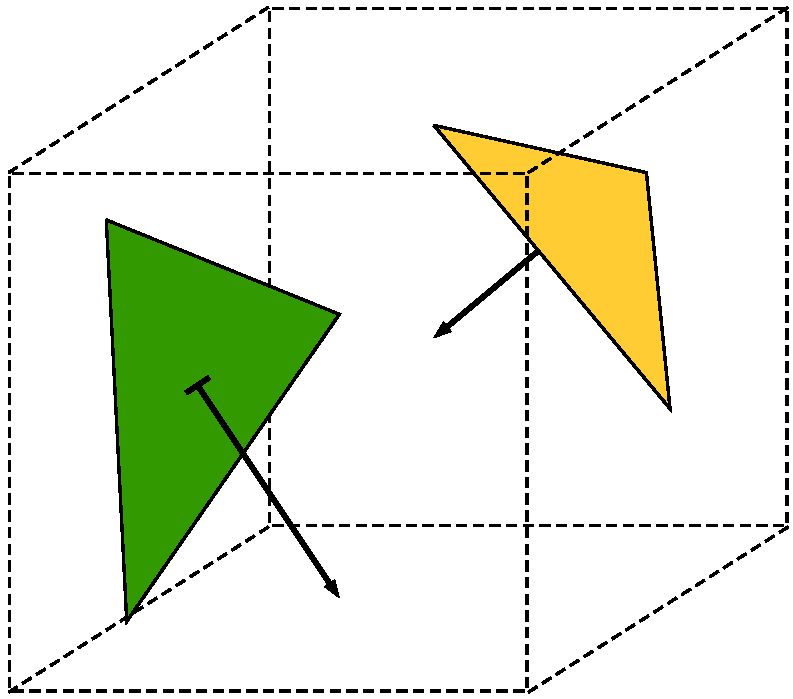
\includegraphics[width=\linewidth]{media/gimped_normals.pdf}
	\caption{Descripción grafica de geometría dentro de un vóxel con normales disparejas.}
	\label{fig:error_normals}
\end{wrapfigure}
Calcular el sombreado de vóxeles de esta forma es suficiente para generar resultados de buena calidad sobre el trazado de conos. Sin embargo uno de los problemas que surgen al simplificar las normales en vóxeles es que algunos vóxeles tienen normales incorrectas o desviadas. Esto sucede especialmente cuando un vóxel contiene geometría con normales muy disparejas. 

Para solventar esto se ideo una alternativa de sombreado sobre la atenuación normal. La idea es calcular la atenuación normal por cada cara del vóxel según la dirección de la luz $\Psi$ y luego ponderar cada atenuación normal por cara con el peso de cada eje en el vector normal. Además del método Lambert tradicional a este método lo llamamos Lambert direccional ponderado. El siguiente código expone su implementación:
\\
\begin{lstlisting}[caption={Sombreado direccional y ponderado según la normal para un vóxel}, label=Shading2]
vec3 BRDF(Light light, vec3 normal, vec3 albedo)
{
    vec3 weight = normal * normal;
    // calculate directional normal attenuation
    float rDotL = dot(vec3(1.0f, 0.0f, 0.0f), light.direction);
    float uDotL = dot(vec3(0.0f, 1.0f, 0.0f), light.direction);
    float fDotL = dot(vec3(0.0f, 0.0f, 1.0f), light.direction);
    // find dominant face
    rDotL = normal.x > 0.0f ? max(rDotL, 0.0f) : max(-rDotL, 0.0f);
    uDotL = normal.y > 0.0f ? max(uDotL, 0.0f) : max(-uDotL, 0.0f);
    fDotL = normal.z > 0.0f ? max(fDotL, 0.0f) : max(-fDotL, 0.0);
    // voxel shading average from all front sides
    nDotL = rDotL * weight.x + uDotL * weight.y + fDotL * weight.z;

    return light.diffuse * albedo * nDotL;
}
\end{lstlisting}

\begin{figure}[H]
	\centering
	\begin{subfigure}[t]{0.2\textwidth}
		\centering
		\captionsetup{justification=centering}
		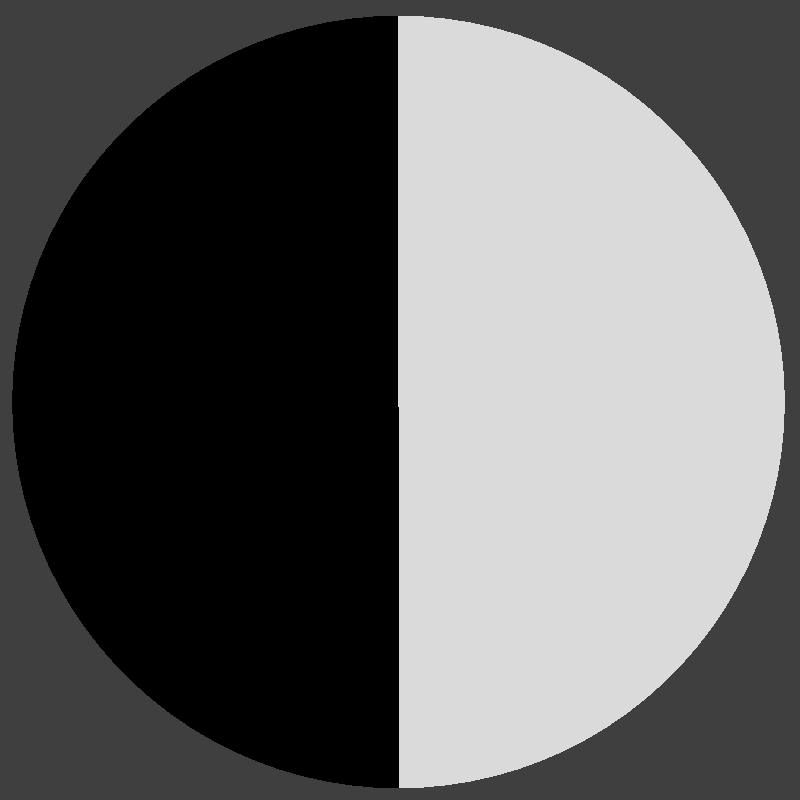
\includegraphics[width=\linewidth]{media/ndotR.png}
		\caption*{Atenuación normal, caras por eje x: \emph{rDotL}}
	\end{subfigure}%
	\begin{subfigure}[t]{0.2\textwidth}
		\centering
		\captionsetup{justification=centering}
		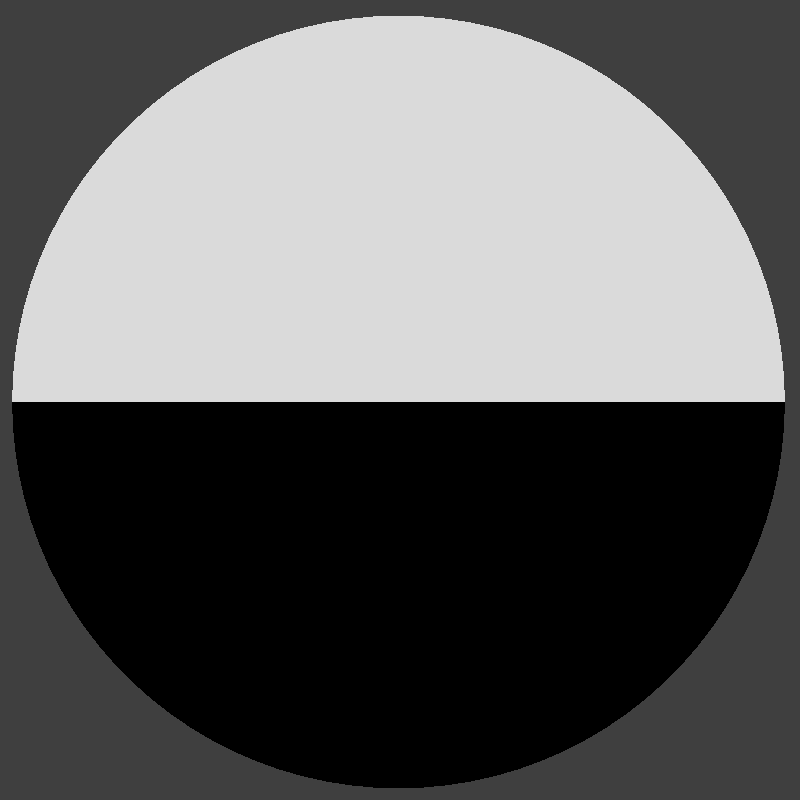
\includegraphics[width=\linewidth]{media/ndotU.png}
		\caption*{Atenuación normal, caras por eje y: \emph{uDotL}}
	\end{subfigure}%
	\begin{subfigure}[t]{0.2\textwidth}
		\centering
		\captionsetup{justification=centering}
		
\includegraphics[width=\linewidth]{media/nDotF.png}
		\caption*{Atenuación normal, caras por eje z: \emph{fDotL}}
	\end{subfigure}%
	\begin{subfigure}[t]{0.2\textwidth}
		\centering
		\captionsetup{justification=centering}
		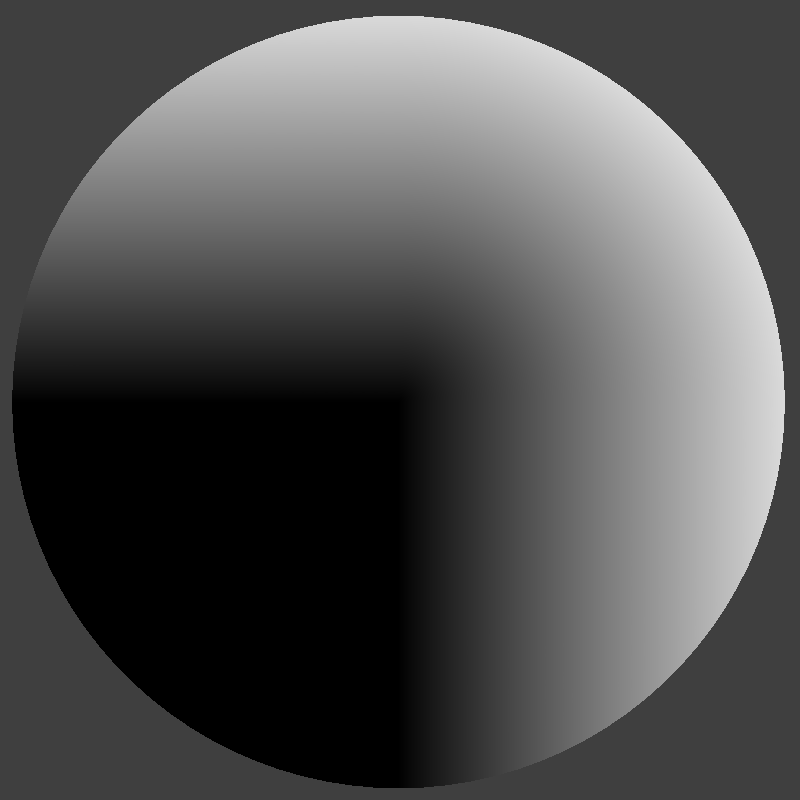
\includegraphics[width=\linewidth]{media/nDotL.png}
		\caption*{Resultado ponderado.}
	\end{subfigure}%
	\begin{subfigure}[t]{0.2\textwidth}
		\centering
		\captionsetup{justification=centering}
		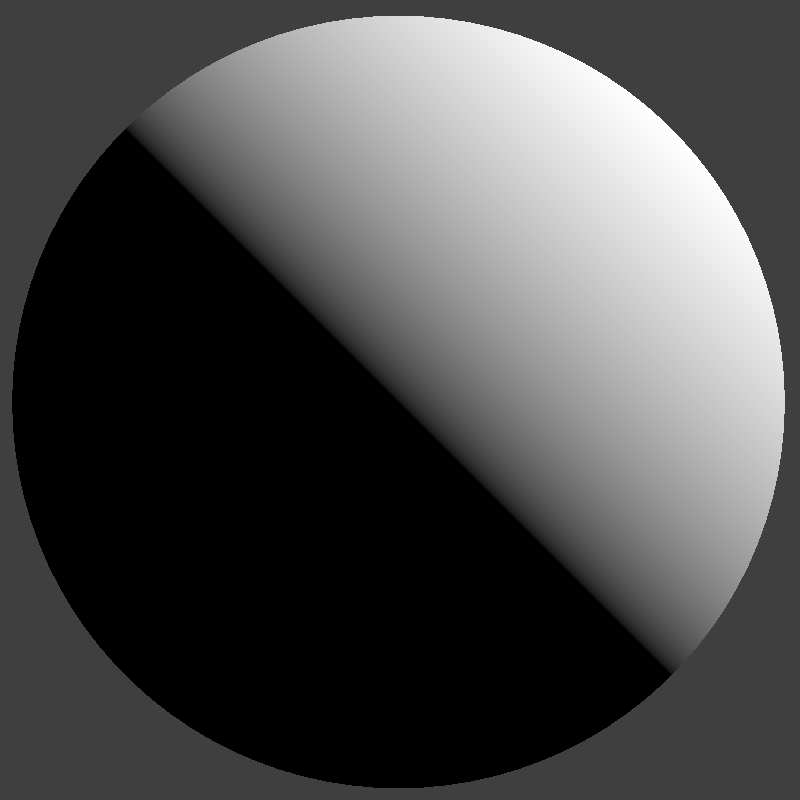
\includegraphics[width=\linewidth]{media/nDotLT.png}
		\caption*{Tradicional.}
	\end{subfigure}%
	\caption{Composición grafica del algoritmo \ref{Shading2} para un ángulo incidente $\Theta$ y $\Psi$ 45 grados en BRDF Explorer \cite{brdf_explorer}.}
	\label{fig:compositve_vshading}
\end{figure}


\subsection{Mapeo y Trazado de Sombras}
\subsection{Vóxeles Emisivos}
% section sombreado_de_vóxeles (end)
